\chapter{Limitations}

Throughout this research Dynamic OpenCL is proven to efficiently compute a variety of algorithms and  execute a multitude of jobs in parallel through a two tiered scheduling infrastructure. Still, in its current version it suffers from several factors that either limit its performance or general functionality.

For instance, while Dynamic OpenCL is deeply rooted to Aparapi and profits from its compelling features it is also limited by it in the complexity of producible code. As explained in section \ref{aparapi} not every Java code can be translated to OpenCL by Aparapi and the respective capabilities of Dynamic OpenCL are therefore tied to Aparapi. Missing features might thus hinder programmers to efficiently write their code or to access low level OpenCL features. Additionally, Aparapi only supports CPUs and GPUs, thus restricting the underlying OpenCL framework that is capable of handling FPGAs and DSPs as well. There have been efforts to allow Aparapi execution on certain FPGAs but none of these modifications have been integrated in the original repository yet\cite{aparapi_ucores}.

While Dynamic OpenCL is able to operate heterogeneous clusters with different hardware vendors and device types, the varying feature sets of devices may become problematic for certain workloads. In section \ref{opencl} an example about the \textit{FP64} feature was portrayed that might be missing for some devices within a cluster. Dynamic OpenCL is currently not able to identify these features and can therefore not schedule appropriately. This means that workloads with a requirement for a specific feature may be assigned to nonsupporting devices and thus produce an error.

During the evaluation Dynamic OpenCL was run for many different cluster compositions and workloads. It is concluded that the network bandwidth is the major limiting performance factor. While this bottleneck is identifiable by the executed benchmarks, another hardware limitation exists that is caused by the architecture of Dynamic OpenCL. In the cluster setup a central node is necessary that manages all running tasks and distributes accompanying data. Throughout the execution of a job it has to hold on to input data while it also receives partial results from the compute nodes. This data has to be kept in memory and in the case of multiple data intense jobs can fill the entire memory. In an appropriate cluster setup the central node should therefore hold sufficient memory to support expected peaks in parallel running jobs. Another strategy is to block further job submissions once memory reaches a certain threshold.

\chapter{Future Work}

In its current state Dynamic OpenCL is a research prototype and therefore still requires significant improvements concerning stability. Additionally, certain features that tackle the previously described limitations of the framework are desirable in the future. While there are numerous potential improvements to the framework, this section covers more substantial topics that can greatly enhance the performance and usability of Dynamic OpenCL.

\section*{Workload Queuing}

\begin{figure}[!htb]	
	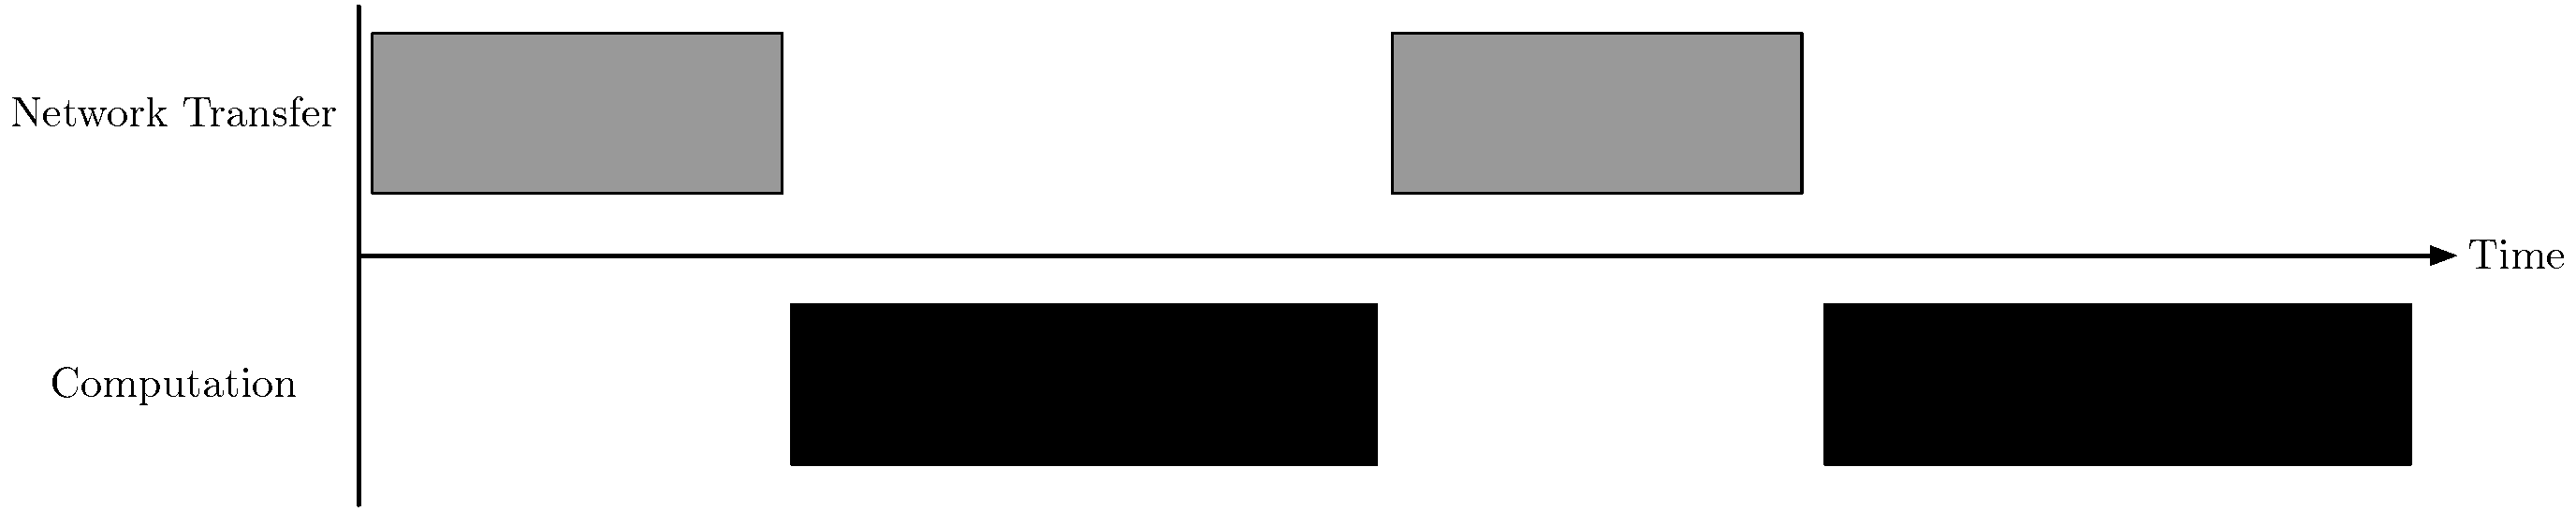
\includegraphics[width=0.85\textwidth]{drawings/missing_queue.pdf}
	\centering
	\caption{Current Execution Workflow}
	\label{img:missing_queuing}
\end{figure}
As shown by the evaluation the overall performance of Dynamic OpenCL is heavily dependent on the available networking capabilities within the cluster. In the current version there might be periods were data transfers to different machines overlap, thus competing for bandwidth. At other times when all devices in the cluster are computing, no data transfers are processed. In figure \ref{img:missing_queuing} the workflow for two subsequent tasks on a compute node is shown. Before the first task can start its data has to be transported to the compute node. As soon as the execution finishes, the output is sent back and the input for its next task is received. During the execution the network connection remains idle. One possibility to improve execution speed of the system is to reduce these idle times and instead use the available bandwidth to transfer data for future tasks. Thus, a subsequent task could start immediately once the previous workload has finished. This way these transfer times would not account to the overall runtime as they would overlap with execution phases. The envisioned workflow is displayed in figure \ref{img:active_queueing}.

\begin{figure}[!htb]	
	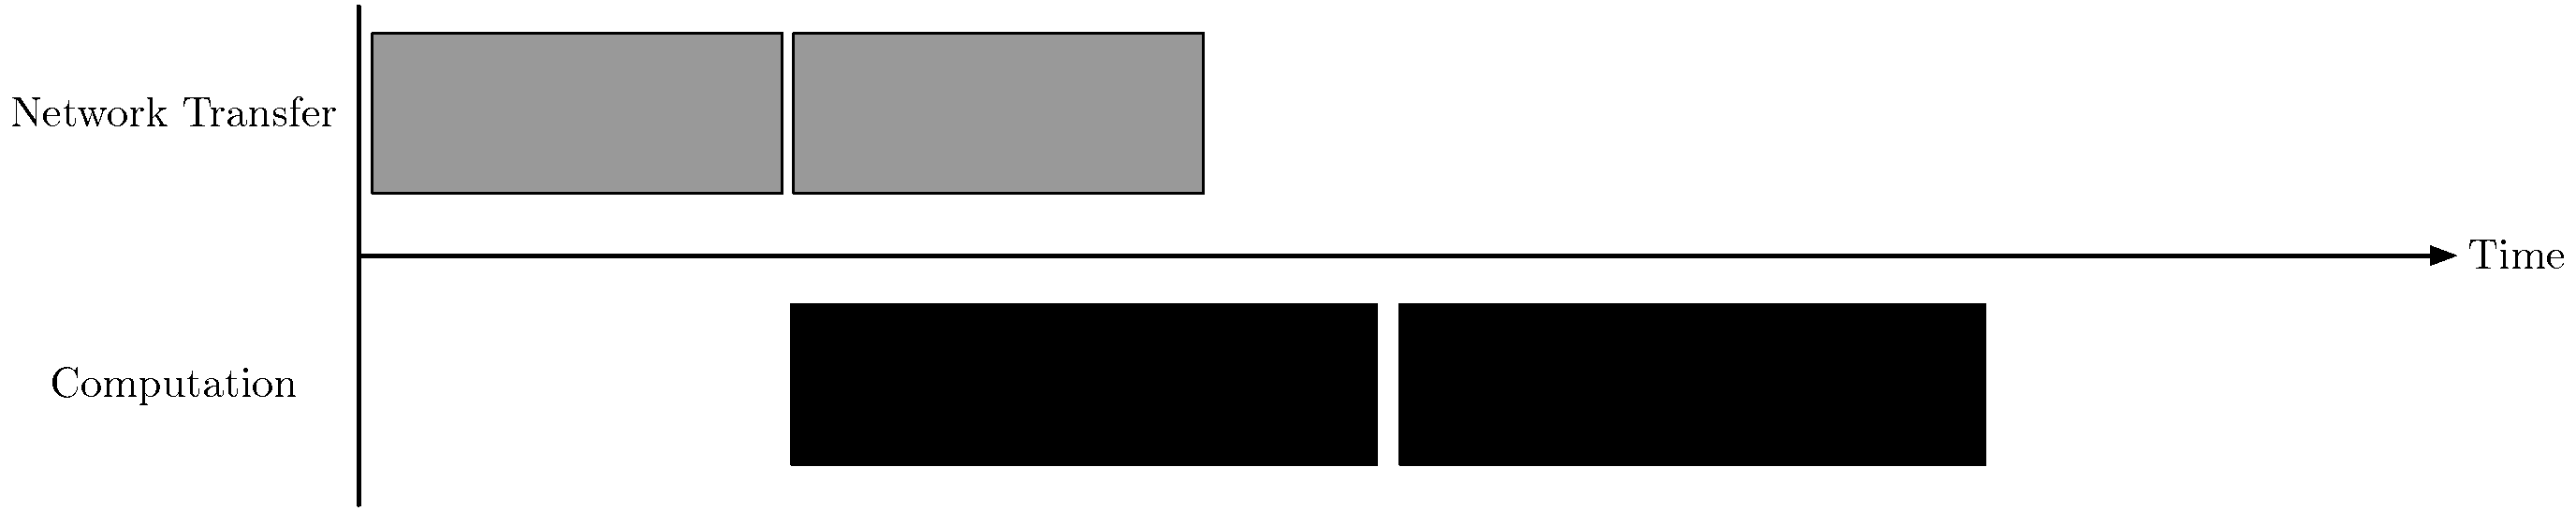
\includegraphics[width=0.85\textwidth]{drawings/active_queue.pdf}
	\centering
	\caption{Future Execution Workflow}
	\label{img:active_queueing}
\end{figure}

In the future workflow once an execution starts the input data of another task can already be transferred, thus queuing that task on the respective machine. Such a mechanism is not trivial to implement. In the given architecture dOpenCL in its current state is only forwarding OpenCL commands. This way it is possible to transfer data buffers to devices that already have another task running. Indeed this may cause memory problems as then two tasks compete for resources on the device and it must be ensured that enough memory is available for both. Instead in the future workflow tasks should be ensured to have entire control over a device without upcoming tasks interfering. It is envisioned to extend dOpenCL by a precaching mechanism that allows to send data buffers to compute nodes beforehand that are held in the main memory or serialized to disk. Once the actual buffer transfer would take place the data is already present on the compute node and only has to be sent from memory to the device.

\section*{Cloud Optimizations}

During the evaluation it was shown that Dynamic OpenCL supports hybrid clusters as well as pure cloud clusters. The prices for the various cloud resources are usually fixed rates. For example each instance type on the EC2 has an \textit{On-Demand} hourly rate that users pay to gain access to an instance for as long as they desire. 

In the current version Dynamic OpenCL supports the manual adjustment of cloud resources. A meaningful feature for users could be the automatic adjustment by the system itself based on deadlines given by the user. For example, when the user submits a job that should be executed within 8 hours, the system might identify that the current computational capabilities are insufficient to reach the deadline. Thus it might book additional cloud resources fitting the actual requirements. Additionally it could recognize certain instance types that perform exceptionally well for a given job and decide to procure more instances of this type.

Another envisioned feature is the optimization of cloud costs by utilizing dynamic pricing features if offered by the respective cloud provider. For example Amazon provides such a feature for its EC2, which is called \textit{Spot Instances}. Heavily underutilized instance types are offered to customers in auctions in which they bid a price they are willing to pay for an instance of a specified type per hour. According to Amazon when their bid is accepted they gain access to the instance for as long as they require the instance or until someone exceeds their bid and no other instances are available in the spot pool\cite{spot_instances}. It was shown by \citeauthor{spot_instance_pricing} that the bidding system is intransparent and that the price is probably not market driven but instead set by an algorithm that is based on other factors like reserve capacity\cite{spot_instance_pricing}. They assume this system is used as the number of spare instances is usually higher than the actual demand, which would result in low spot prices that are uneconomical for Amazon. 
\begin{figure}[!htb]	
	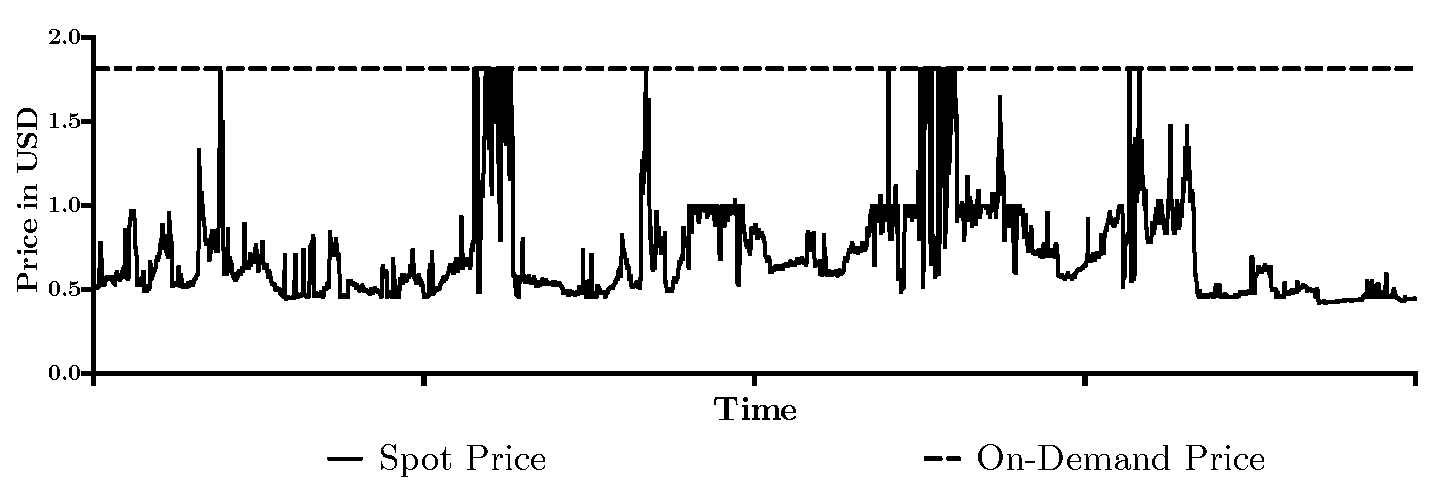
\includegraphics[width=0.7\textwidth]{images/ec2_spot_prices.pdf}
	\centering
	\caption{EC2 Spot Price Rate for c4.8xlarge Instances}
	\label{img:spot_pricing}
\end{figure}
Nevertheless spot instances offer strong discounts over on-demand prices as shown in figure \ref{img:spot_pricing}, which depicts real historic prices for a week. The on-demand price fluctuates strongly below the on-demand barrier, at times reaching values that are 23\% of the on-demand price. Utilizing historic data and knowledge about Amazon's pricing algorithm, Dynamic OpenCL could indicate users when to book spot instances for cheaper job executions or make these decisions automatically.

\chapter{Conclusion}

In this research Dynamic OpenCL is introduced, which represents a framework for distributing parallel computations among multiple machines within a cluster. Its development is based on goals defined in section \ref{goals}. Dynamic OpenCL allows to utilize \textit{heterogeneous} compute devices by employing OpenCL as its underlying computational framework. Thus, CPUs and GPUs of various vendors can be used that make it possible to efficiently process \textit{diverse workloads}. Distributing workloads across a cluster is enabled by dOpenCL, which allows to access remote devices without changes to the OpenCL code. Aparapi is added to the framework in order to allow users an \textit{ease of programming} by writing OpenCL Kernels in Java. Additionally Dynamic OpenCL introduces its own execution model in which computations are split into partials, which can be executed in parallel on multiple devices. Dynamic OpenCL also allows to dynamically \textit{scale resources} by adding cloud resources to the cluster. An extendable scheduling architecture is utilized for \textit{scaling execution speeds} of jobs. Different scheduling algorithms also allows to adapt to complex cluster setups like hybrid clusters in order to provide an \textit{optimized scheduling} solution.

The extensive evaluation shows that Dynamic OpenCL is able to operate various cluster setups and allows efficient execution for mixed workloads. In all portrayed environments the framework yields significant improvements to performance when employing additional machines. It is shown that the individual achievable speedups are dependent on the data intensity of the respective workloads as well as the available network bandwidths. Even in a heavily bottlenecked scenario of a hybrid cluster, remote cloud resources can assist computations noticeably when employing a suitable scheduling strategy. Aside from pure performance considerations, Dynamic OpenCL also enables cluster administrators to reach better hardware utilization by dynamic resource adjustments. This may lead to individual monetary benefits by reducing the total cost of ownership for hardware.

Overall Dynamic OpenCL allows users access to distributed cluster computations at a high abstraction level. Not only does it offer inexperienced users to overcome the steep learning curve of OpenCL but also aids seasoned programmers to develop their programs faster by eliminating OpenCL boilerplate code. In order to harness parallel compute resources, programmers may split their datasets manually into partials, which is deemed to be intuitive in an object oriented environment like Java. 

Dynamic OpenCL is conceived with adaptability in mind regarding cloud services. As such it can be adjusted to new upcoming cloud providers with minor changes. Additionally, cloud provides like Amazon are currently introducing novel resource types like FPGAs\cite{amazon_fpga}. Utilizing these devices is possible by the underlying OpenCL model but is currently not supported by Aparapi. Thus, harnessing these powerful devices still requires additional work to Dynamic OpenCL.
